\documentclass[10pt,twocolumn]{article}

\usepackage[a4paper,margin=0.75in]{geometry}
\usepackage{booktabs}
\usepackage{enumitem}
\usepackage{graphicx}
\usepackage[hidelinks]{hyperref}
\usepackage{tikz}
\usetikzlibrary{arrows.meta,positioning}

\pagestyle{plain}

\title{VisionGuard: Local Computer Vision for Gesture Recognition and Continuous User Authentication}
\subtitle{Bachelor Semester Project S2, University of Luxembourg}

\author{Stefan Penchev}
\email{stefan.penchev.001@student.uni.lu}
\affiliation{%
  \institution{University of Luxembourg}
  \city{Esch-sur-Alzette}
  \country{Luxembourg}
}

\author{Bereket A. Yilma}
\email{bereket.yilma@uni.lu}
\affiliation{%
  \institution{University of Luxembourg}
  \city{Esch-sur-Alzette}
  \country{Luxembourg}
}

\begin{document}

\begin{abstract}
This project creates a local desktop system for gesture recognition and continuous user authentication.
The system uses a camera to observe the user, records gesture samples, trains a small recognition model, and runs live inference while the desktop application is active.
When a trained gesture is detected with enough confidence, the application can execute a mapped desktop action, such as opening an application, changing volume, sending a keyboard shortcut, or performing a mouse click.
The project is built as a modular system with an Electron and React desktop interface, a TypeScript shared contract layer, and a Python FastAPI service for datasets, training jobs, model status, hand-presence checks, and gesture inference.
The aim is to show how local computer vision can support secure and practical interaction without sending camera data to a remote service.
\end{abstract}

\noindent\textbf{CCS Concepts:}
Human-centered computing~--~User interface toolkits;
Computing methodologies~--~Computer vision;
Security and privacy~--~Authentication.

\medskip
\noindent\textbf{Keywords:}
Computer Vision, Gesture Recognition, Continuous Authentication, Electron, React, FastAPI, MediaPipe, Human-Computer Interaction, Local AI.

\maketitle

\section{Introduction}
Modern desktop systems still depend mainly on keyboards, touchpads, passwords, and short authentication checks.
These inputs work well for many tasks, but they do not always match situations where the user needs fast interaction, hands-free control, or continuous confidence that the right person is operating the system.
Camera-based computer vision can help with this problem because it allows the system to observe gestures and user presence without requiring a separate physical controller.

VisionGuard explores this idea through a local desktop application.
The system connects a live camera view with gesture recording, gesture training, model monitoring, and action execution.
Instead of only asking whether the user logged in once, the application is designed around an ongoing security workflow: the camera session is started, the user records gestures, the model is trained from local samples, and live inference checks whether the current movement matches a known gesture.

The project focuses on a practical balance between usability and control.
The user can define gestures, choose what action each gesture should trigger, review sample thumbnails, send the gesture to training, and then monitor model state during live use.
The system does not replace traditional authentication.
Instead, it shows how local computer vision can become an additional layer for user verification and workstation control.

\section{Related Work}
\subsection{Gesture Recognition}
Gesture recognition systems try to understand hand or body movement from sensor data.
Traditional systems often used depth cameras, wearable sensors, or handcrafted image features.
More recent approaches use machine learning and landmark detection to extract richer information from normal camera input.
MediaPipe Hands is an example of a widely used hand-tracking pipeline that can detect hand landmarks in real time and support interactive applications \cite{zhang2020mediapipe}.

Gesture recognition is useful in human-computer interaction because it can reduce friction in tasks where keyboard and mouse input is slow or inconvenient.
For a desktop system, gestures can act as shortcuts for repeated actions.
However, the system must also avoid accidental activations.
This is why confidence thresholds, cooldown periods, and clear event feedback are important parts of the design.

\subsection{Continuous Authentication}
Continuous authentication checks user identity or user behavior after the initial login step.
Instead of trusting a session forever, the system keeps collecting evidence that the active user still matches the expected user.
Research in this area includes keystroke dynamics, mouse behavior, face recognition, gait, touch patterns, and multimodal approaches \cite{patel2016continuous}.

VisionGuard is related to continuous authentication because it treats camera input as an ongoing signal.
The current implementation concentrates on gesture recognition and user-presence workflow rather than full biometric identity verification.
Still, the architecture leaves space for a continuous-authentication model family alongside gesture recognition.

\subsection{Local AI and Privacy}
Camera-based systems can introduce privacy risks because video frames may contain faces, rooms, documents, or other sensitive context.
For this reason, local processing is an important design choice.
In VisionGuard, the desktop application and AI service run on the same machine.
The camera frames and sample files are handled locally, and the model service is accessed through a local URL.
This reduces reliance on remote processing and gives the user more direct control over the data flow.

\section{Background}
\subsection{Why Gesture Control Needs Reliability}
Gesture control is useful only when it is predictable.
A gesture that fails too often becomes frustrating, while a gesture that triggers too easily becomes unsafe.
This is especially important when gestures are connected to desktop actions such as keyboard shortcuts or mouse clicks.
The system therefore needs a clear training workflow, a visible model state, and a confidence threshold before execution.

\subsection{Why Authentication Needs More Context}
Passwords and login screens usually check identity at one point in time.
After that, the computer often assumes that the same person remains in control.
In shared rooms, labs, or workstations, this assumption can be weak.
Continuous authentication adds context by checking signals during the session.
VisionGuard uses the camera as the first input channel for this kind of context.

\subsection{Project Constraints}
The project was built as a local desktop prototype.
The current desktop action support targets macOS because it uses platform commands such as \texttt{open} and \texttt{osascript}.
The AI service is implemented as a Python service running on \texttt{127.0.0.1:8765}.
The interface can render in a browser for development, but gesture actions, file persistence, and inference integration are intended for the Electron desktop environment.

\section{Project Objectives}
This project creates a local computer-vision application for secure and efficient desktop interaction.
The main goals of the project are:

\begin{itemize}[leftmargin=*]
  \item Build a desktop interface where the user can start a camera session and monitor camera state.
  \item Allow users to record gesture samples and map each gesture to a desktop action.
  \item Store gesture samples locally and send structured sample references to an AI service.
  \item Train a gesture-recognition model from captured samples.
  \item Run live inference against camera frames and show prediction confidence.
  \item Execute desktop actions only when the prediction confidence is high enough.
  \item Keep the architecture modular so gesture recognition and continuous authentication can evolve independently.
\end{itemize}

The system is designed to support the user, not to hide decisions from them.
The interface shows model health, training status, camera state, prediction output, and recent events so the user can understand what the system is doing.

\section{Methods}
This section explains how VisionGuard was built.
The system combines desktop development, local web technologies, and Python computer-vision processing.

\subsection{System Design Approach}
The system follows a modular design.
Each part has a clear responsibility and communicates through typed contracts.
The three main ideas are:

\begin{enumerate}[leftmargin=*]
  \item \textbf{Local processing:} Camera frames, gesture samples, training jobs, and inference requests stay on the local machine.
  \item \textbf{Typed integration:} The desktop app and AI service use a shared contract for datasets, training jobs, model status, and inference results.
  \item \textbf{User-centered control:} The user records gestures, reviews captured samples, starts training, and sees model and event feedback.
\end{enumerate}

\subsection{Technical Setup}
VisionGuard has three main technical parts:

\begin{itemize}[leftmargin=*]
  \item \textbf{Desktop application:} Electron, React, TypeScript, Vite, and Lucide React are used to build the user interface and desktop bridge.
  \item \textbf{Shared kernel:} A TypeScript package defines the AI model service contract used by the desktop layer.
  \item \textbf{AI service:} Python, FastAPI, OpenCV, NumPy, and MediaPipe support dataset creation, hand-presence checks, model training, and inference.
\end{itemize}

\subsection{Architecture Overview}
Figure \ref{fig:architecture} shows the main system flow.
The renderer captures camera frames and samples, Electron stores local files and calls the AI service, and the AI service manages datasets, training jobs, model artifacts, and inference responses.

\begin{figure}[t]
\centering
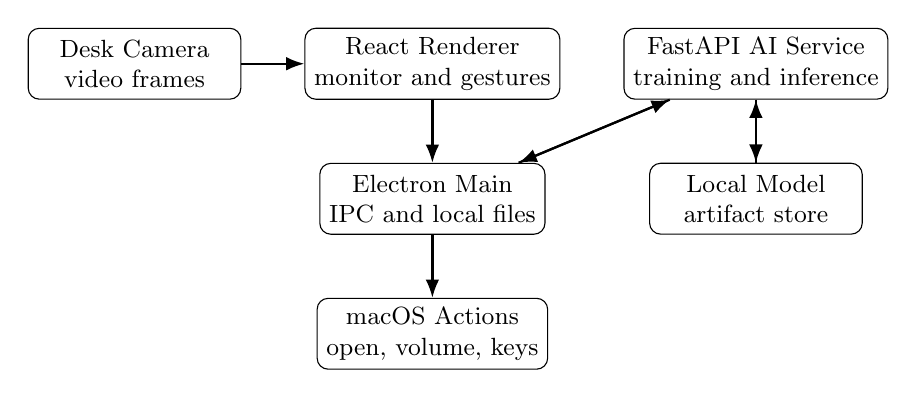
\begin{tikzpicture}[
  node distance=8mm,
  box/.style={draw, rounded corners, align=center, minimum width=2.7cm, minimum height=0.9cm, font=\small},
  arrow/.style={-Latex, thick}
]
\node[box] (camera) {Desk Camera\\video frames};
\node[box, right=of camera] (renderer) {React Renderer\\monitor and gestures};
\node[box, below=of renderer] (electron) {Electron Main\\IPC and local files};
\node[box, right=of renderer] (service) {FastAPI AI Service\\training and inference};
\node[box, below=of service] (model) {Local Model\\artifact store};
\node[box, below=of electron] (actions) {macOS Actions\\open, volume, keys};

\draw[arrow] (camera) -- (renderer);
\draw[arrow] (renderer) -- (electron);
\draw[arrow] (electron) -- (service);
\draw[arrow] (service) -- (model);
\draw[arrow] (model) -- (service);
\draw[arrow] (service) -- (electron);
\draw[arrow] (electron) -- (actions);
\end{tikzpicture}
\caption{VisionGuard architecture: local camera frames pass through the Electron application to the local AI service, which returns training and inference results.}
\label{fig:architecture}
\end{figure}

\section{System Framework}
\subsection{Framework Overview}
The VisionGuard workflow has four main stages.
First, the user starts a camera session.
Second, the user records gesture samples and saves them as a gesture definition.
Third, the saved gesture is sent to the AI service for training.
Fourth, live inference uses the trained model to detect gestures and trigger desktop actions.

\begin{figure*}[t]
  \centering
  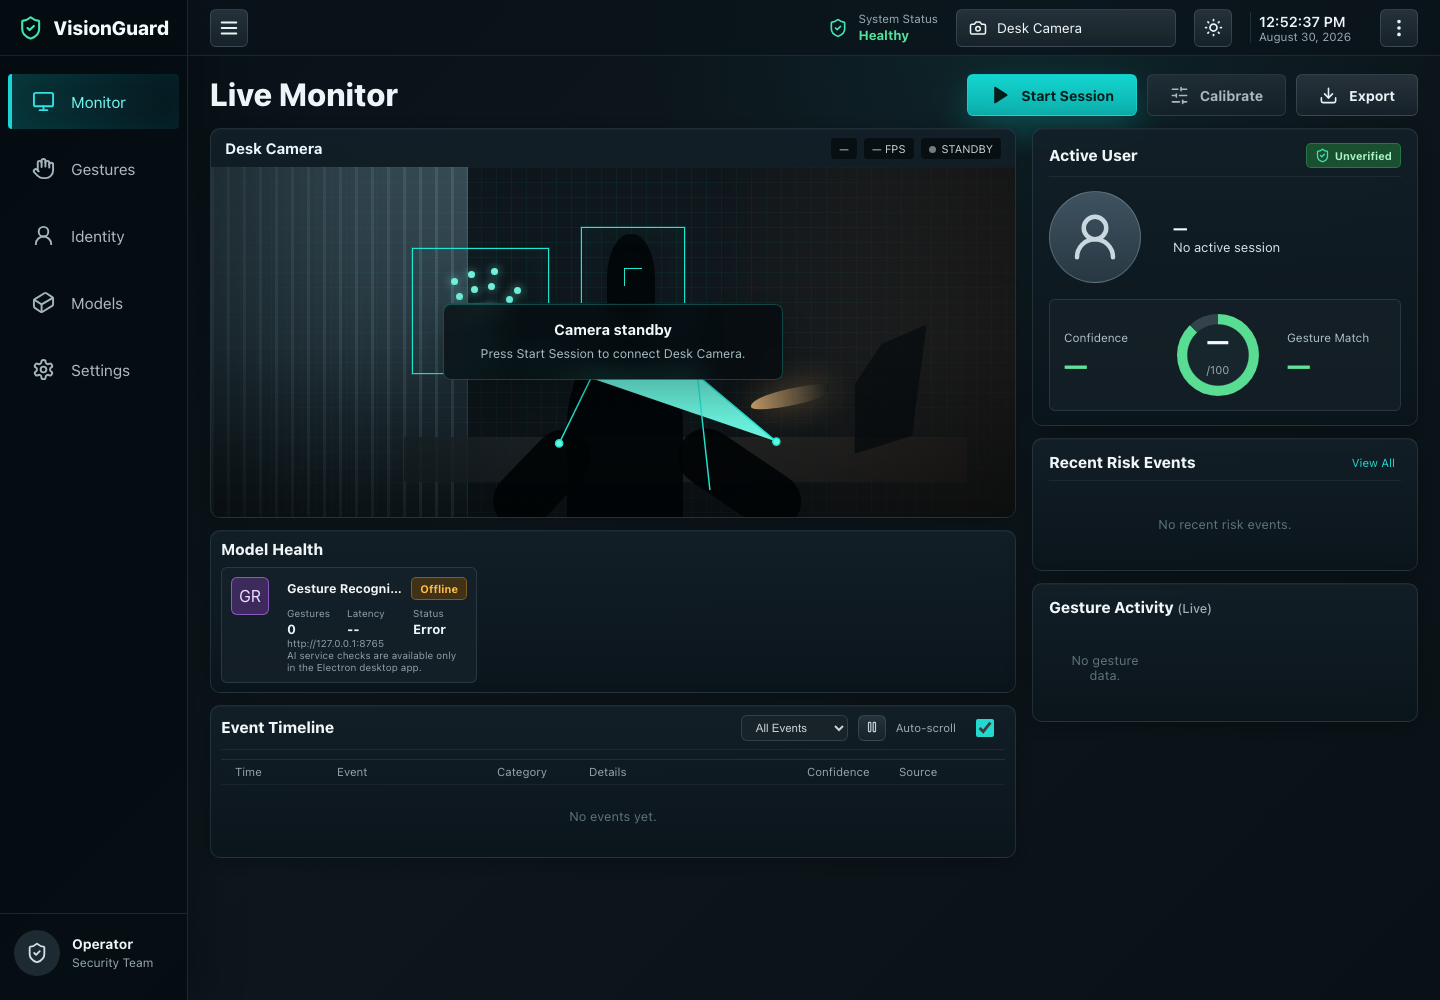
\includegraphics[width=\textwidth]{figures/visionguard-monitor.png}
  \caption{VisionGuard live monitor screen. The interface shows camera state, model health, user verification state, gesture activity, and the event timeline.}
  \label{fig:monitor}
\end{figure*}

\subsection{Stage 1: Camera Session}
The camera session is the starting point of the system.
The user selects a camera and presses \textit{Start Session}.
When the camera is active, the interface shows the live preview, camera resolution, frame rate, and readiness state.
If the camera is inactive, the monitor shows a standby illustration and explains that the user must start a session.

\subsection{Stage 2: Gesture Recording}
The gesture panel allows the user to create a new gesture.
The user chooses an action type, enters a gesture name, enters an action target, and records samples.
The application expects 12 valid samples before the gesture can be saved.
During capture, the system checks whether a hand is present in the frame.
This prevents empty or unusable samples from entering the training dataset.

\begin{figure*}[t]
  \centering
  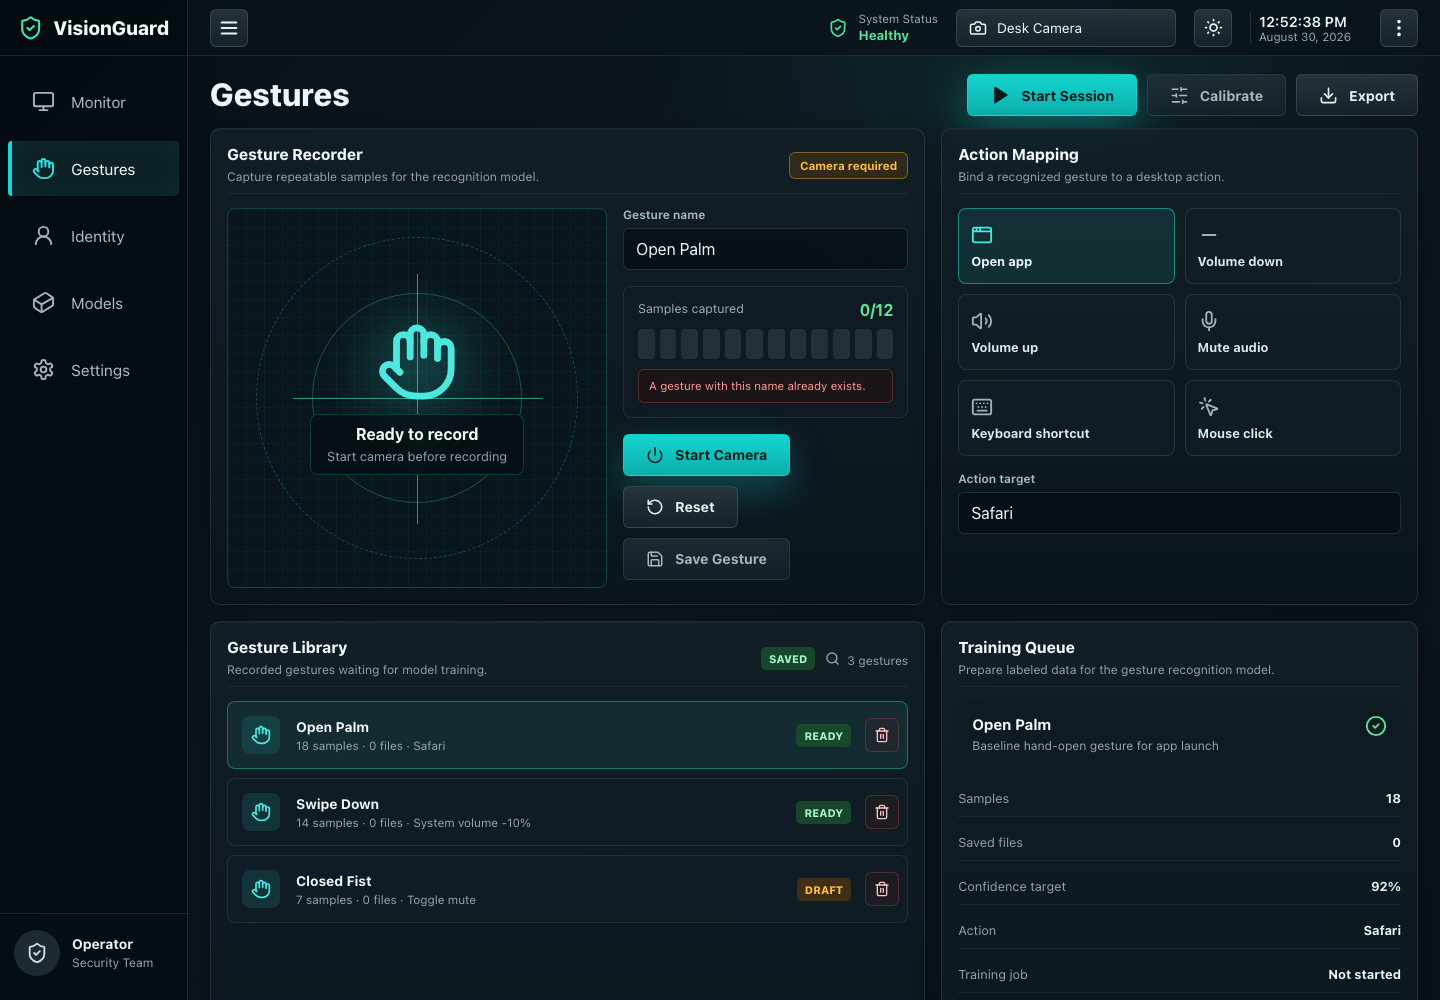
\includegraphics[width=\textwidth]{figures/visionguard-gestures.png}
  \caption{Gesture recording and training interface. The user maps a gesture to an action, captures samples, saves the gesture, and sends it to training.}
  \label{fig:gestures}
\end{figure*}

\subsection{Stage 3: Training}
When a gesture is ready, the user can send it to training.
Electron sends the gesture labels and sample references to the AI service.
The AI service creates a dataset, starts a training job, updates progress, and saves a model artifact in the local model directory.
The desktop app polls the training job and updates the gesture status when the job is completed, failed, or cancelled.

\subsection{Stage 4: Live Inference and Action Execution}
Live inference runs only when the camera is active, at least one gesture is trained, the AI service is online, and the model status is ready.
The renderer captures frames periodically and sends them through Electron to the AI service.
The AI service returns predictions with confidence values.
If the best prediction matches a trained gesture and the confidence is high enough, the desktop layer executes the mapped action.
The current action confidence threshold is 0.92, and a cooldown period prevents one gesture from repeatedly triggering the same command.

\section{System Building}
\subsection{Technology Stack and Architecture}
The desktop app is built with a modern TypeScript stack.
React is used for the renderer interface, Electron provides access to desktop capabilities, and Vite supports development and build tooling.
The AI service is implemented with FastAPI.
Computer-vision work uses OpenCV and MediaPipe for hand-related processing.
The project is organized as a workspace with separate packages for the desktop app, shared contracts, and AI service.

\subsection{Custom Building Components}
\subsubsection{Live Monitor}
The live monitor is the main operating screen.
It shows the camera preview, model health, event timeline, active-user panel, and gesture activity.
This screen is designed for repeated use because the user needs to quickly understand whether the system is ready, offline, training, or waiting for a gesture.

\subsubsection{Gesture Library}
The gesture library stores gesture definitions with names, action types, targets, confidence goals, sample counts, and training state.
The current application supports actions for opening an application, reducing volume, increasing volume, muting audio, sending a keyboard shortcut, and clicking the mouse.

\subsubsection{AI Service Contract}
The shared contract defines the data shapes used across the desktop app and AI service.
Important objects include \texttt{TrainingDataset}, \texttt{TrainingJob}, \texttt{ModelStatus}, \texttt{InferenceResult}, and \texttt{HandPresenceResult}.
This keeps the desktop and Python service aligned even though they are implemented in different languages.

\subsubsection{Hand-Presence Detection}
Before a sample is accepted, the system checks whether a hand is visible.
The Python worker uses MediaPipe hand detection and additional image-processing methods to locate likely hand regions.
This makes the training set cleaner because the application avoids saving frames where the user has not shown a hand.

\subsubsection{Desktop Actions}
The Electron main process executes desktop actions after a confident match.
On macOS, the implementation uses system commands to open apps, adjust volume, toggle mute, send keyboard shortcuts, or issue a mouse click.
If the platform is not macOS, the action layer returns an error instead of pretending that the command worked.

\subsection{Example Data Flow}
Table \ref{tab:dataflow} shows a simplified example of the system data flow during one gesture-training cycle.

\begin{table}[t]
  \caption{Example gesture-training data flow}
  \label{tab:dataflow}
  \centering
  \begin{tabular}{lll}
    \toprule
    Step & Component & Output \\
    \midrule
    Capture & Renderer & JPEG frame sample \\
    Validate & AI service & Hand detected or rejected \\
    Save & Electron main & Local sample reference \\
    Dataset & AI service & Training dataset ID \\
    Train & AI worker & Model artifact path \\
    Monitor & Renderer & Ready model state \\
    \bottomrule
  \end{tabular}
\end{table}

\begin{figure*}[t]
  \centering
  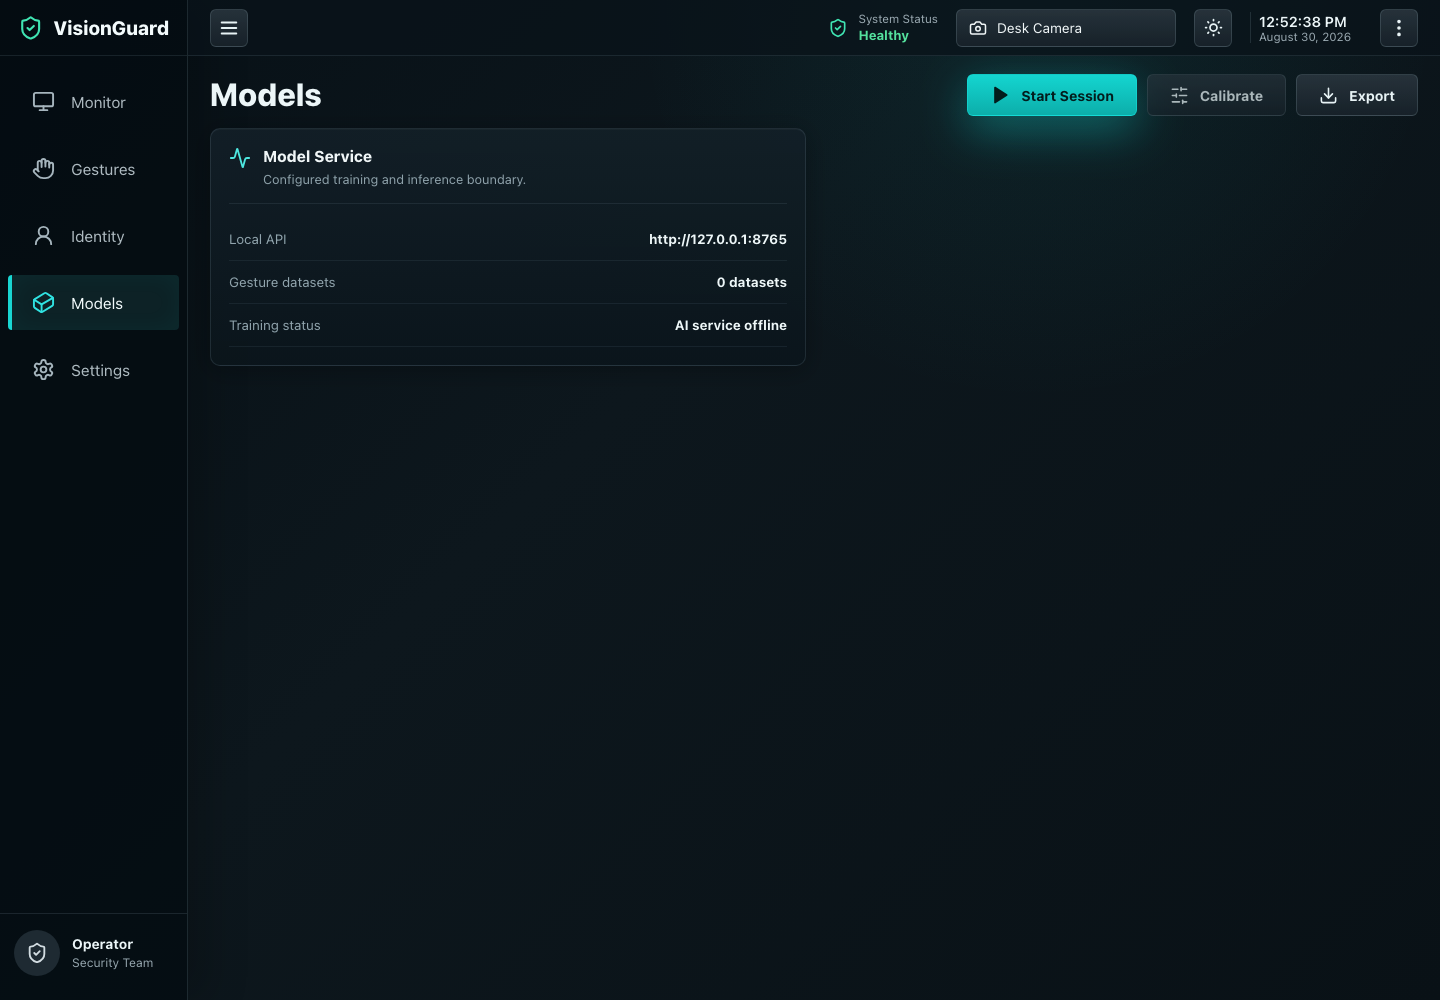
\includegraphics[width=\textwidth]{figures/visionguard-models.png}
  \caption{Model and secondary views. The application separates model status, identity context, and settings from the main monitor workflow.}
  \label{fig:models}
\end{figure*}

\section{Results}
\subsection{Functional Results}
The project reached the following main results:

\begin{itemize}[leftmargin=*]
  \item A working Electron desktop interface for camera monitoring and gesture management.
  \item A gesture recorder that captures samples and checks hand presence before saving.
  \item A local AI service with endpoints for datasets, training jobs, model status, hand detection, and inference.
  \item A shared contract layer between the desktop app and AI service.
  \item A live inference workflow that connects predictions with action execution.
  \item A dashboard that reports model health, inference state, and recent events.
\end{itemize}

\subsection{Security and Privacy Relevance}
VisionGuard is relevant because it keeps sensitive camera processing local.
The system does not require a cloud service to train or run gesture inference.
This is important because camera frames may contain personal information.
The project also shows that authentication-related features should be visible and explainable.
The user can see whether the system is online, whether a model is trained, whether inference is ready, and what action was triggered.

\section{Conclusion}
This project shows that a local computer-vision workflow can support gesture recognition and continuous authentication concepts in a desktop application.
The system combines an Electron and React interface with a Python FastAPI AI service.
It records gesture samples, validates hand presence, trains a local gesture model, runs live inference, and triggers desktop actions only after a confident prediction.

VisionGuard is still a prototype, but it provides a complete foundation for future work.
The most important contribution is the end-to-end connection between user-facing camera workflows and local AI model operations.
This makes the system practical to test and extend.

\section{Future Work}
\subsection{Stronger Continuous Authentication}
The current application includes identity and model-family concepts, but the main implemented workflow is gesture recognition.
A future version can add face recognition, behavioral signals, or multimodal scoring to support stronger continuous authentication.

\subsection{Improved Gesture Model}
The gesture model can be improved with richer landmark features, temporal motion features, and better calibration.
A stronger model should compare not only one frame but also short sequences so that dynamic gestures such as swipes can be recognized more accurately.

\subsection{Cross-Platform Action Support}
Desktop action execution is currently implemented for macOS.
Future work can add Windows and Linux support through platform-specific adapters.
This would make the application useful in more environments while keeping each platform implementation explicit.

\subsection{Dataset and Model Persistence}
The current AI service stores training state in memory while model artifacts are written locally.
A future version can persist datasets, jobs, metrics, and model metadata in a structured database.
This would make the system more reliable across restarts and easier to audit.

\subsection{Evaluation}
The next step is to evaluate the system with repeated gesture trials.
Useful metrics include detection accuracy, false activation rate, training time, inference latency, and user-perceived usability.
This would make it possible to compare different models and thresholds.

\section*{Acknowledgments}
I would like to thank Pr. Dr. Bereket A. Yilma for guidance, feedback, and support during the development of this project.
The project benefited from discussions about system architecture, human-centered design, and applied machine learning.

\begin{thebibliography}{9}

\bibitem{zhang2020mediapipe}
Fan Zhang, Valentin Bazarevsky, Andrey Vakunov, Andrei Tkachenka, George Sung, Chuo-Ling Chang, and Matthias Grundmann.
\newblock 2020.
\newblock MediaPipe Hands: On-device real-time hand tracking.
\newblock In \textit{Workshop on Computer Vision for AR/VR at CVPR}.

\bibitem{patel2016continuous}
Vishal M. Patel, Raghuraman Chellappa, Deepak Chandra, and Brandon Barbello.
\newblock 2016.
\newblock Continuous user authentication on mobile devices: Recent progress and remaining challenges.
\newblock \textit{IEEE Signal Processing Magazine} 33, 4 (2016), 49--61.

\bibitem{opencv}
Gary Bradski.
\newblock 2000.
\newblock The OpenCV Library.
\newblock \textit{Dr. Dobb's Journal of Software Tools}.

\bibitem{electron}
Electron Contributors.
\newblock 2026.
\newblock Electron documentation.
\newblock \url{https://www.electronjs.org/docs}

\bibitem{fastapi}
Sebastian Ramirez.
\newblock 2026.
\newblock FastAPI documentation.
\newblock \url{https://fastapi.tiangolo.com/}

\end{thebibliography}

\end{document}
